% \documentclass[oneside]{report}
\documentclass[oneside,final,14pt,a4paper]{extreport}
% \documentclass[journal,onecolumn,a4paper,12pt]{IEEEtran} 

% \usepackage[T2A]{fontenc}
\usepackage[T1]{fontenc}
\usepackage{textcomp}

\usepackage{fontspec}
\setmainfont{Times New Roman}
% \setmonofont[Scale=0.9]{Courier}

\usepackage{vmargin}
\setpapersize{A4} 
\setmarginsrb{2.5cm}{2cm}{2cm}{2cm}{0pt}{10mm}{0pt}{13mm}
\usepackage{setspace}
\sloppy
\setstretch{1.5}
\usepackage{indentfirst}
\parindent=1.25cm

%%%%% ADDED TO SUPPORT TT BOLD FACES %%%%
% \DeclareFontShape{OT1}{cmtt}{bx}{n}{<5><6><7><8><9><10><10.95><12><14.4><17.28><20.74><24.88>cmttb10}{}

% \renewcommand{\ttdefault}{pcr}
% \usepackage{courier}

%%%%% END %%%%%%%%%%%%%%%%%%%%%%%%%%%%%%% 
% \usepackage{atbegshi,picture}
% \AtBeginShipout{\AtBeginShipoutUpperLeft{%
%   \put(\dimexpr\paperwidth-1cm\relax,-1.5cm){\makebox[0pt][r]{
\includegraphics[width=3cm]{figs/inno}}}%
% }}
 

\usepackage[english]{babel}
\usepackage[backend=biber,style=ieee,autocite=inline]{biblatex}
% \addbibresource{ref.bib}
\bibliography{ref.bib}
\DefineBibliographyStrings{english}{%
  bibliography = {References},}
\usepackage{blindtext}
\usepackage{pdfpages}
\newenvironment{bottompar}{\par\vspace*{\fill}}{\clearpage}
\usepackage{amsmath,amsfonts}

\usepackage{amsthm}
\newtheorem{theorem}{Theorem}
\newtheorem{corollary}{Corollary}
\newtheorem{lemma}{Lemma}
\newtheorem{proposition}{Proposition}
\theoremstyle{definition}
\newtheorem{definition}{Definition}
\theoremstyle{remark}
\newtheorem*{remark}{Remark}
\theoremstyle{remark}
\newtheorem*{example}{Example}

\usepackage{float}
\usepackage{graphicx}
\graphicspath{{figs/}} %path to images
\usepackage{array}
\usepackage{multirow,array}
\usepackage{caption}
\usepackage{subcaption}
\usepackage{hyperref}
\usepackage{paralist}

\usepackage{listings}
\lstset{basicstyle=\ttfamily,breaklines=true}

\usepackage{zed-csp}
\usepackage{fancyhdr}
\usepackage{color}

\usepackage{upgreek} 
\usepackage{bm}
\usepackage{hyperref}
\usepackage{setspace}
\usepackage{booktabs}
\usepackage{multirow}
\usepackage{longtable}
\usepackage[font=singlespacing, labelfont=bf]{caption}
\counterwithout{table}{chapter}
\renewcommand{\thetable}{\Roman{table}}
%Hints
\newcommand\pic[1]{(Fig. \ref{#1})} %Ref on figure
\newcommand\tab[1]{(Tab. \ref{#1})} %Ref on table

\setlength{\headheight}{17.0pt}


\usepackage{enumitem}
\newlist{inlinelist}{enumerate*}{1}
\setlist*[inlinelist,1]{%
  label=(\arabic*),
}

\usepackage[nopygments]{ffcode}
\usepackage{csquotes}





\pagestyle{fancyplain}

% remember section title
\renewcommand{\chaptermark}[1]%
	{\markboth{\chaptername~\thechapter~--~#1}{}}

% subsection number and title
\renewcommand{\sectionmark}[1]%
	{\markright{\thesection\ #1}}

\rhead[\fancyplain{}{\bf\leftmark}]%
      {\fancyplain{}{\bf\thepage}}
\lhead[\fancyplain{}{\bf\thepage}]%
      {\fancyplain{}{\bf\rightmark}}
\cfoot{} %bfseries


\newcommand{\dedication}[1]
   {\thispagestyle{empty}
     
   \begin{flushleft}\raggedleft #1\end{flushleft}
}

\usepackage{subfiles}

\begin{document}

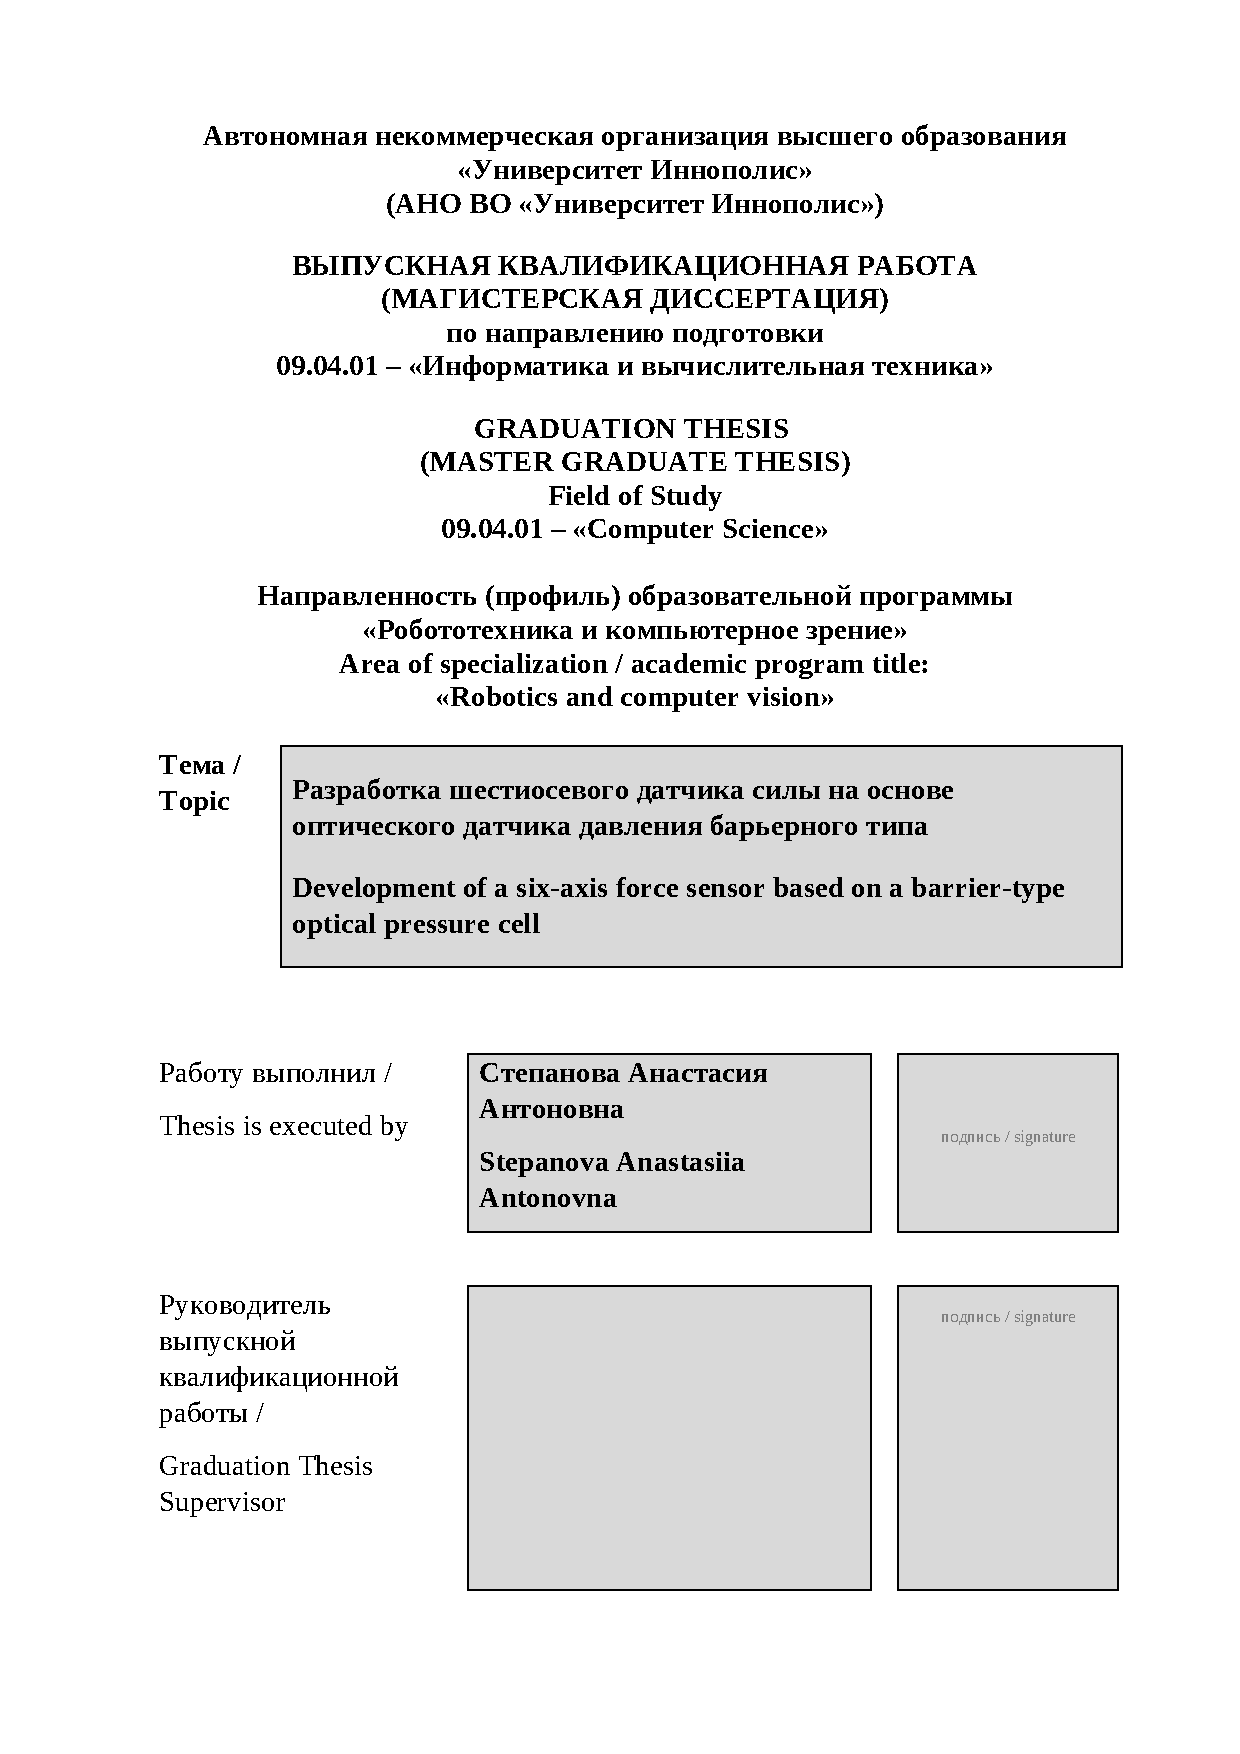
\includepdf[pages=-, offset=75 -75]{title.pdf}
\tableofcontents
% \listoftables
% \listoffigures


\newpage
\begin{abstract}
\label{abstract}

The multi-axis force sensor market is currently dominated by strain gauge sensors, but other options exist, such as hall-effect, fiber Bragg grating (FBG), and optoelectronic cells. 


The optoelectronic cell is perceptible due to its low cost, excellent precision, and simple implementation. Nevertheless, a dearth of solutions appropriate for large-scale manufacturing and enable adjustable sensor parameters exists.


This study aims to explore how the shape and material of the barrier affect the measurement range of an optoelectronic barrier-type sensor. Additionally, a modular multi-axis force sensor will be designed using the measurement cells.


The study design involves examining the impact of barrier shape and material on the measurement range of the optoelectronic barrier-type sensor. Additionally, in the research, I designed a modular multi-axis force sensor based on the presented measurement cells.


The optoelectronic six-axial force sensor, which is the focus of this study, is characterized by its simplicity and ease of implementation as a modular sensor. It provides a cost-effective solution and facilitates the straightforward replacement of construction elements.
 Consequently, this sensor has the potential to broaden the range of applications for multi-axis force sensors.

This research contributes to understanding how the shape and material of the barrier affect the measurement range of optoelectronic barrier-type sensors. The design of a modular multi-axis force sensor provides a cost-effective and adjustable solution for various robotic applications.
\end{abstract}
% Depend on above part
\setcounter{page}{7}

\chapter{Introduction}
\label{chapter:introduction}


% BACKGROUND
Multi-axial force sensors, also referred to as multi-axis force sensors, are devices that can measure forces and torques in multiple directions or axes simultaneously (from one to six dimensions). 
These sensors find applications in various fields such as robotics, biomechanics, and industrial automation \cite{multi_axis_force_sensors_review}. 

% There are different types of multi-axial force sensors available, each utilizing different sensing technologies. 
% The strain-gauge sensor is commonly used in this field, but optical sensors have shown higher accuracy and linearity \cite{perfect_sensor}.

% Novelty/Research Gap/Unknown
The classical multi-axis force sensor is a system of uniaxial pressure sensors of different dimensions.
While the strain-gauge sensor remains the most common solution as uniaxial pressure measurement cell in the field of multi-axial force sensors, 
optical sensors shows noticeable accuracy with higher linearity \cite{perfect_sensor}. 
The structures of the optical multi-force sensors has been solid \cite{perfect_sensor, 1990_optic}, while for strain-gauge based sensors fully mechanically decoupled solutions exists \cite{decoupling_sliding_structure, modal_sensor}. 

% Questions/Problems/Purpose of study
The objective of this project is to investigate the relationship between the linearity of optical sensors 
and the construction of the barrier and multi-axial sensor configuration.
% Experimental/Design Approach
The project is divided in two parts: development of a single degree of freedom pressure sensor and a multi-axis force sensor based on a designed pressure cell.
Both parts aim to develop a mathematical model for the sensor, its prototype and conduct testing to evaluate accuracy, hysteresis and axis crosstalk.
% I decided to held experiments under normal conditions and calibrate the sensor under statical load.

% A bridge to LR
The multiaxis force sensor development is ...


The most common solutions for multi-axial force sensors constructions and pressure cells types are described in the  


% By doing so, we hope to contribute to the existing body of knowledge in the field of force sensor technology.


% Не актуально из-за высокой стоимости калибровки датчика. добавить про актуальность, цену датчика и шум, сказать что на оптопарах есть предположение 
% что можно сделать дешевле. В конце посчитать сколько стоит производство такого датчика (партии).

% прописать задачи^ мат модель, зависимость, разработать прототип одноосевого, проверить эксперементально модель, разработать шестиосевой. 
% Прототип на фотополимерном принтере.

% квадратный барьер, разработка экспериментов (калибровка в нормальных условиях, измерение точности и гистерезиса).
% после цели, задачи, плавный переход в литревью.
% на магистерскую оптимизация формы барьера с учетом элестостатических показателей статики формы крышки.

\section{Overview of thesis contents}

\nameref{chapter:literature_review} chapter will outline the general information about multi-axial force sensors, force measurement cells technologies and state pros and cons of multi-axial force sensors existing solutions. 
Also the chapter will review methods of statical calibration and experimental setups used for testing the sensor' kind.

\nameref{chapter:optical_modeling} chapter will provide the mathematical model of the optical force measuring cell.

Construction modeling will present the target multi-axis sensor structure.

In \nameref{chapter:implementation} chapter I describe the experimental setup and the results evaluation techniques, provide comparison with my mathematical model.

% \nameref{chapter:results_and_discussion} chapter will outline the outcome of the sensor and discuss the future possibilities of the project.
% Java Overview chapter will describe the source language structure and most notable features that matter for the project.

% EO Overview chapter will outline the target language structure and most notable features that matter for the project.

% Implementation chapter will provide projecting methodology in depth, as well as describe the project implementation details.

% Results and Discussion chapter will present the outcome of the implemented project and discuss the future possibilities and relevance of the project.

\chapter{Glossary}
\label{chapter:glossaries}

\begin{tabular}{>{\bfseries}r l}
    cell of a sensor & ...\\
    coupling & ... \\
    crosstalk & undesired measured output of a\\
     &transverse channel under defined load \\
     &on the calibrated axis ISO 21612:2021(E) \\
    cross-coupling & ... \\
    isotropy & exhibiting properties (such as velocity of \\
    &light transmission) with the same values \\
    &when measured along axes in all directions \cite{isotropic}\\
    ERSG & Electrical Resistance Strain Gauge\\
    FBG & Fiber Bragg grating\\
    % isotropy & qux \\
    % modal & qux \\
    % deaerators & \\
    Data acquisition (DAQ) & the process of measuring an electrical\\
    & or physical phenomenon, such as voltage, current, \\
    & temperature, pressure, or sound. 
standards.
\end{tabular}

% ISO standard ISO 21612:2021(E) : https://cdn.standards.iteh.ai/samples/71244/7382a3ec26df41158157474b764c33c8/ISO-21612-2021.pdf


% \glossary{Указатель : упорядоченный перечень объектов текста ,
% благодаря чему можно быстро находить сведения об этих
% объектах, когда требуется справка или выборочное чтение
% издания}
% \glossary{Глоссарий : собрание глосс, предшественник словаря }
% \glossary{ xindy | i s {программа для формирования вспомогательного
% указателя, может использоваться и для создания глоссария }}
% \glossary{ xindy | s e e {Указатель }}
% \glossary{ xindy | s e e a l s o {Глоссарий }}

% % Печать готового глоссария gl s −файла
% \printglossary{}
\chapter{Literature Review}
\label{chapter:literature_review}

\section{Navigation}
\label{lr_navigation}


% задачи
% рассказать про решения, сделать вывод, почему именно оптические датчики силы. Добавить цифры для типов ячеек. почему оптобарьерный. Потом уже структуры.
%  открываю стандарт на датчики силы, смотрю на терминологию. В интродакшену к литревью указать источник терминологии + указать на проюлему в терминах.

% Добавить часть с калибровкой и базовыми параметрами для датчиков силы.(мб в самом начале, давать термины, указать, как они измеряются). Потом про типы датчиков по типу измерения, потом конструкции.

The objective of this chapter is to conduct a literature review on the development of six degrees of freedom (DOF) force sensors. 
Section \ref{lr_pressure_cell_types} defines the types of pressure sensors used as measurement cells for multi-axis force and torque sensors, 
along with their limitations. 
In Section \ref{lr_constructions}, an examination of the construction of multi-axial load sensor beams is presented. 
% Section 2.4 focuses specifically on photointerrupter pressure cells and investigates the measurement techniques proposed
%  for them. 

% \ref{lr_calibration} The current section focus on the decoupling methods based on calibration. 

Finally, in Section \ref{lr_conclusion}, the research gap in this field is identified.
\section{Pressure cells types}

\label{lr_pressure_cell_types}
% датчики стресса и 
% добавить пьезоэлектрический датчик, добавить 
\subsection{Piezoresistors}
\subsection{Capacitive sensor}
The capacitance of a flat capacitor can be determined using equation (\ref*{eq:capacitance}). 
This formula describes the connection between capacitance, plate area, and the distance between the plates of the device. 
Changes in distance and area result in variations in capacitance, which is utilized in capacitance-based pressure sensors to measure changes in distance.
The principle is as follows: when pressure is applied to the capacitor's plate and alters the distance $d$, the changes in capacitance are measured and converted into a signal.
\begin{equation}
    \label{eq:capacitance}
    C = \frac{\varepsilon_0 \varepsilon A}{d}
\end{equation}
\begin{figure}[t]
    \centering
    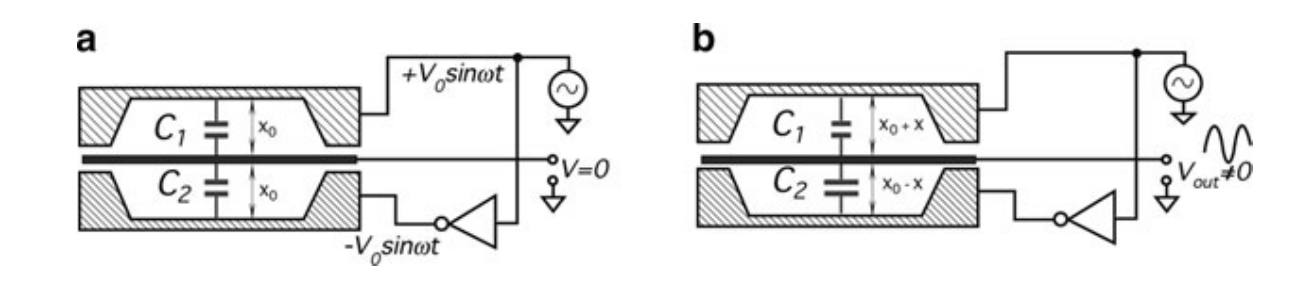
\includegraphics[width=\textwidth]{/LR/capacitive_sensors.png}
    \caption{Principle of operation for a flat-plate capacitive sensor. Adapted from \cite[Fig. 7.6]{handbook_sensors}.}
    \label{fig:capacitive_sensors}
\end{figure}

Capacitive sensors can be monopolar, differential (utilizing two capacitors), or a capacitive bridge can be utilized (using four capacitors) \cite{handbook_sensors}.
A typical capacitive pressure sensor is differential, with a diaphragm surface serving as the central plate, as depicted in Fig. \ref*{fig:capacitive_sensors}, creating a dual variable capacitor \cite{pressure_sens_calibration_stat_dyn}.
The capacitance changes when a load is applied to the diaphragm surface. 

Capacitive pressure sensors have broad measurement range, high sensitivity, accuracy and reliability, absence of contamination risk, large range of working temperatures (-70 \textdegree C to 400 \textdegree C).
The sensors are low-cost, highly sensitive devices mostly used in exceptional circumstances, such as miniature or even MEMS force sensors \cite*{multi_axis_force_sensors_review} and harsh environmental conditions.

\subsection{Electrical Resistance Strain Gauge}
The principle behind Electrical Resistance Strain Gauges (ERSGs) is the change in resistance caused 
by deformation, as explained in a study by official representative of Keller AG manufacturer \cite{keller_article}. 
Stretching or compressing of the piezoresistive material results in a change in the electric resistance of the sensor 
\cite{multi_axis_force_sensors_review}. 
% When the piezoresistive material is stretched or compressed, 
% it results in a change in the electric resistance of the sensor 
% \cite{multi_axis_force_sensors_review}. 
In order to accurately measure small changes in geometry, 
strain-gauge sensors are typically connected to a Wheatstone bridge.

Since the creation of the multi-axis force sensor in the 1970s, 
the strain-resistive pressure sensor has remained a classic measuring device \cite{3d_FBG_sensor}. 
However, these solutions tend to be expensive and require additional surface treatment of the substrate, 
as well as high-quality technology for bonding with a strain-resistant component 
\cite{my_love_pressure_photosensor, fingertip_based_FBG}. Load cells, which utilize strain gauges, 
face challenges in signal processing. These challenges include sensitivity to temperature and magnetic noise, 
the need for regular calibration, and difficulties in maintenance after the substrate undergoes plastic deformation.
% TODO: rephrase
Regarding response times, typical values of this measuring principle range from 1 to 10 ms. \cite{pressure_sens_calibration_stat_dyn}

\subsection{Fiber Bragg grating}
Fiber Bragg gratings (FBG) are the most popular optical pressure measurement methods. The FBG sensor is a specific type 
of distributed Bragg reflector that is created within a short section of optical fiber. 
Its function is to selectively reflect certain wavelengths of light while allowing all other wavelengths to pass through. 
When subjected to strain or temperature variations, the reflected wavelengths of an FBG shift accordingly. 
The magnitude of this wavelength shift is directly proportional to the applied load.
Several scientific papers, including Xiong L. et al. \cite{3d_FBG_sensor} and Guo Yu \cite{fingertip_based_FBG}, 
have documented the development of six-axis force sensors utilizing a fiber Bragg lattice. 
This design offers several advantages over strain-resistant sensors, such as immunity to electromagnetic interference, 
a compact profile, and lightweight construction. However, important to note that FBG-based sensors 
necessitate significant investments in optical signal demodulation equipment \cite{3d_FBG_sensor}, 
as well as surface treatment processes.

\subsection{Photointerrupter cell with barrier}

The optocoupler pressure sensor comprises three main components: a light emitter, two light receivers, and an interrupter positioned between emitter and one of the receivers \cite{my_love_pressure_photosensor}. 
When a load is applied to the sensor, the interrupter plate shifts, thereby altering the rate of light intensity on the measuring diode \cite{1990_optic}.
The signal from the second receiver is a reference and enables the cancellation of the optocoupler characteristics change, that effects whole system equally, caused by temperature, dirt and etc.

In the mathematical model of this type of cell, the barrier can be considered as a spring, making the applied force proportional to the deformation of the barrier.

This type of sensor has negligible hysteresis and repeatability error, since the vane movement amplitude to close the measuring diode is very small \cite*{pressure_sens_calibration_stat_dyn}.
Additionally, it offers a compact geometry and is cost-effective. % Moreover, since the optical surface usually is 

Compared to ERSG sensors, the photointerrupter measurement cell is less susceptible to electrical interference \cite*{my_love_pressure_photosensor}. 

The properties associated with hysteresis and the sensor's nominal range are primarily influenced by the type of barrier utilized \cite{my_love_pressure_photosensor}.
\begin{figure}[t]
\centering
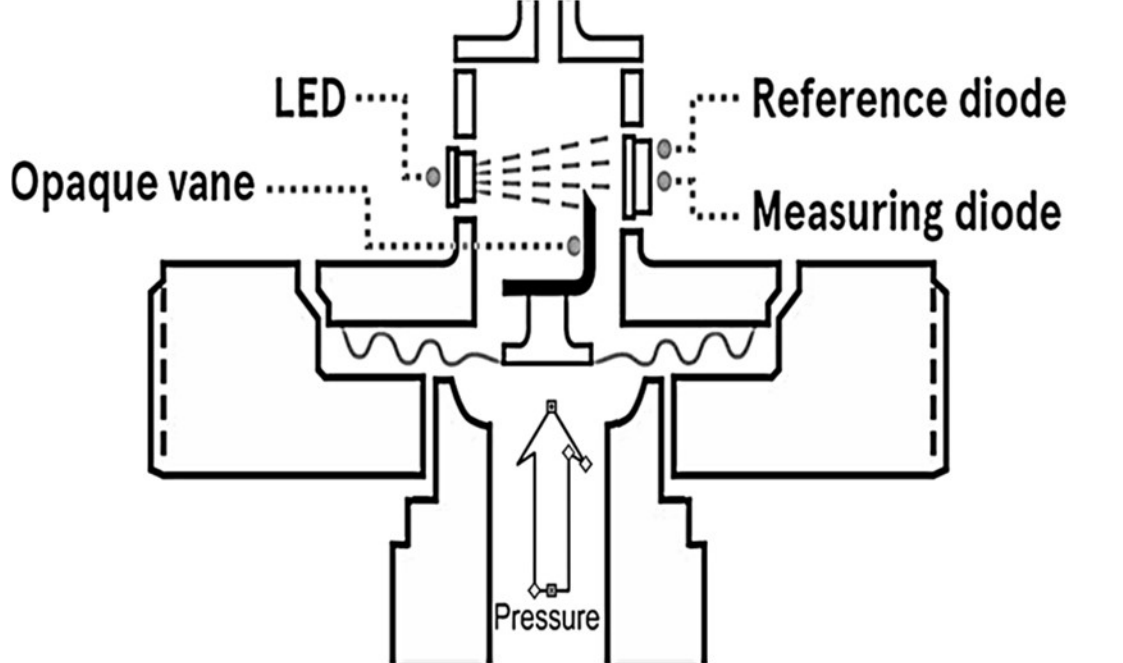
\includegraphics[width=0.5\textwidth]{optical_force_sensor.png}
\caption{Example of an optical pressure sensor. Adapted from \cite[Fig. 5]{pressure_sens_calibration_stat_dyn}.}
\label{fig:optical_sensor_arrangement}

\end{figure}

% TODO: rephrase
Other advantages of this type of pressure sensor that are particularly important in some industrial applications are its long transmission distance and the low chemical reactivity of the material, which is ideal
for operating in environments with a risk of explosion, in addition to being intrinsically safe [25]. Regarding response time, typical values of this measuring principle can reach values about $100 \mu$s. \cite{pressure_sens_calibration_stat_dyn}

% TODO: rephrase
In terms of force, the sensor has an average resolution of 0.1 N over a 200 N measurement range \cite*{OPTIC_CELL_FOR_HAND}.

% TODO: continue
The described characteristics of the sensor type force me to use the one in the research and try to apply the measurement principle in cells of my multi-axial force sensor.

\section{Metrics}
stiffness, nominal values, isotropy
In a coupled sensor an axis force component produces signal in more then one measurement cell, therefore calibration becomes more complicated.
% Add hysteresis graphs.  взять из учебника.
% isotropy - какой контекст
%  взять характеристики датчика из учебника, которые подходят. Прочитать раздел с датчиками силы.
\subsection{Coupling}
\label{lr_coupling}

One of the main metrics for multi-axial force sensor is degree of coupling, which determines the complexity of calibration matrix of a sensor 
\cite{decoupling_sliding_structure,multi_axis_force_sensors_review,CHAO1997105}. 
Dimensions coupling problem is one of the most common problems for multi-axial force sensors \cite{NN_decoupling}.
The degree of coupling among the axes directly impacts the accuracy of the sensor and the complexity of calibration 
\cite{decoupling_sliding_structure, multi_axis_force_sensors_review, CHAO1997105}. 
In a coupled sensor, an axis force component can produce signals in more than one measurement cell, 
thereby complicating the calibration process. However, designing and manufacturing highly decoupled structures can be challenging 
\cite{shape_optimization_decoupled}.

To reduce axis dependence one may change structure of the sensor or perform high precision calibration. 
Existing solutions for multi-axial force sensor structures are presented in the \ref{lr_constructions} section.

\section{Calibration}
\label{lr_calibration}
The multi-axis calibration has static and dynamic methods based on the applied force/pressure \cite{Static_Dynamic_Calibration_FlexiForce, pressure_sens_calibration_stat_dyn}.
A load usually is said to be static, if it remains constant during the measurement process. Accordingly, a load is said to be dynamic if it varies significantly in a short amount of time, usually, several times during the measurement.
The dynamic calibration is applied to sensors designed for highly dynamic environment with pressure pulsations or to determine the sensor response time \cite{pressure_sens_calibration_stat_dyn}. 
In my research the static calibration is sufficient, therefore, lets focus on the methods used in the multi-axis force sensors development.

Two static calibration methods exists: traditional and neural-networks based \cite{NN_decoupling, Deep_Learning_Calib}. % the first one writes about decoupling aka calibration - dummy article btw

Traditional method involves linear transformation (LT) of pressure cells output to the force and torque space using least-square-method (LSM) \cite{Deep_Learning_Calib}.
The mapping is represented with $N\times6$ matrix, where $N$ - number of uniaxial pressure sensors of the system \cite{Deep_Learning_Calib}.
The method defines two limitations \cite{Deep_Learning_Calib}:

\begin{itemize}
    \item The LT defines the linear dependency of sensor' output to the elastic body transformation.
    \item Matrix mapping representation requires load axes independence. 
\end{itemize}

% Нагнетание датчика мб надо добавить
In other words, the sensor output has to be linear to applied load with fully decoupled axes. 
The conditions are hard to satisfy, therefore many researches about structural sensors decoupling exists \cite{beam_structure_math,decoupling_sliding_structure,shape_optimization_decoupled,modal_sensor}.

Neural-networks based 

\dots

\subsection{How the ISO standart determines the calibration process}

— All force and moment channels are measured during the calibration process of each axis. All channels
are to be offset corrected in unloaded condition prior to the calibration test.

For force loading the force is applied within the neutral axes of the load cell.

In order to keep accuracy and to prevent  misalignment it should be avoided to exert torque within the mounting plane between load cell and fixture. This load case should be last in the sequence. It can cause rotation of the load cell within the fixture. Thus subsequently exerted loads can be shifted from the intended load axis

\subsubsection{misalignment determination}

For a loading in discrete steps or a continuous loading procedure, the output voltages in [mV/V] of all
transverse channels need to be recorded.
After the calibration of all axes, the current sensitivities of these channels are known and can be used
for the calculation of the crosstalk as percentage of the transducer axis’ calibration range.
For the force and moment channels, the transverse channels’ output voltage recorded in [mV/V]
(see NOTE 1) shall be converted to the physical dimension force or moment by applying the current
sensitivity determined from the calibration test before. 


\section{Constructions}
\label{lr_constructions}

Typically, the assessment of forces and moments in various directions is achieved by utilizing multiple strain-sensitive sensors affixed to a 
flexible substrate \cite{multi_axis_force_sensors_review}. The structure of a sensor plays a crucial role in its design as it governs 
characteristics such as stiffness, nominal values, isotropy, and the coupling among the measured axes 
\cite*{multi_axis_force_sensors_review,beam_structure_math}. 

To create optimized decoupled structures, engineers employ finite element analysis (FEM) 
\cite*{1990_optic, multi_axis_force_sensors_review, beam_structure_math}.

% Typically, the assessment of forces and moments in various directions is carried out through the 
% utilization of multiple strain-sensitive sensors that are affixed to a flexible substrate\cite{multi_axis_force_sensors_review}.
% The structure of a sensor is an essential component of its design, as governs characteristics such as stiffness, nominal values, isotropy, and the coupling among 
% the measured axes \cite*{multi_axis_force_sensors_review,beam_structure_math}. The last one determines the accuracy of the sensor and calibration complexity \cite{decoupling_sliding_structure,multi_axis_force_sensors_review,CHAO1997105}. 
% In a coupled sensor an axis force component produces signal in more then one measurement cell, therefore calibration becomes more complicated. 
% Nevertheless, the high-decoupled structures are hard to design and manufacture \cite{shape_optimization_decoupled}. 
% To create optimized decoupled structure engineers use finite element analysis (FEM) \cite*{1990_optic,multi_axis_force_sensors_review,beam_structure_math} 
% and with computational power growth creation of mechanically decoupled solutions becomes easier. 
% In their study Mayetin and Kucuk \cite{modal_sensor} created a modal sensor with average average interference error <3\%. The approach allows to replace failed structural elements.

% A multi-axis force sensor with a high coupling level 
% The configuration determines strain distribution and the position of the sensors \cite{beam_structure_math}. 
% In the multi-axis force sensors review \cite{multi_axis_force_sensors_review} authors proposed categorization for elastic structure designs.
% The types of six DOF force sensors structures: six DOF cross-beam, column-type, beam-column type, Stewart platform. Brief descriptions of each beam structure are in the next subsections.

% \subsection{Six DOF cross-beam structure}

\begin{enumerate}
    \item Rigid jointed cross-beams
\end{enumerate}
The most prevalent type of sensors used are rigid-joined sensors, primarily due to their solid beam structure, 
which facilitates simplified manufacturing. 
According to studies conducted by \cite{multi_axis_force_sensors_review, beam_structure_math}, 
rigid-joined cross beams exhibit reduced measurement isotropy and an increased level of coupling. 
The high level of coupling of rigid-joined sensors pushed researchers to find mechanically decoupled solutions.
A comprehensive compilation of rigid-joined cross-beam sensors can be found in \cite{multi_axis_force_sensors_review}.

\begin{enumerate}[resume]
    \item Flexible jointed cross-beams
\end{enumerate}

% TODO: Add reference to the figure flexible_beams
The flexible jointed structure was created to avoid the calibration complexity of mechanically coupled sensors \cite{shape_optimization_decoupled}. 
Want is a flexible joint of the cross-beam? Some researches define the flexible joint as a thin regions in the beam structure. 
Those regions are elastic compared to the whole beam, therefore they act as a damper and reduce the cross dimension coupling. 

The second type of flexible jointed cross-beams is the $WHICH_WORD_TO_USE$. Their constructions has additional mechanical component as joint, for example, bearings or hinges.

\begin{figure}[H]
    \begin{subfigure}[b]{0.3\textwidth}
        \label{fig:flexible_beams_a}
        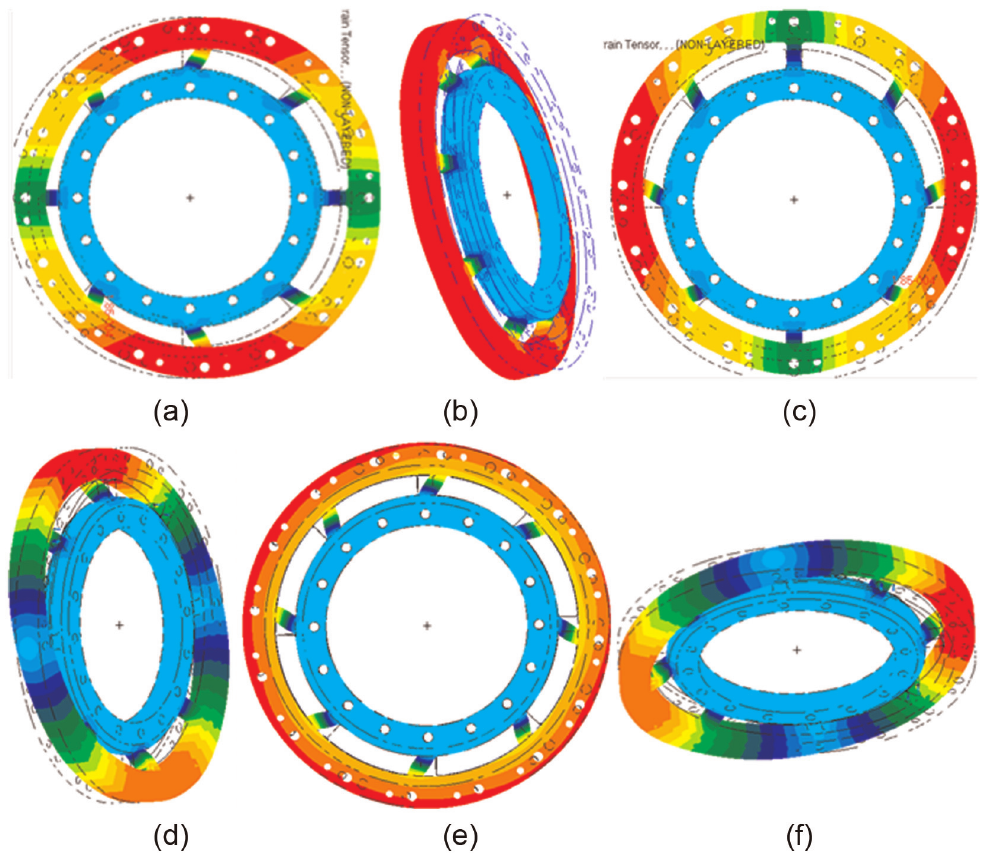
\includegraphics[width=\textwidth]{flexible_beam.png}
        \caption*{thin joints}
    \end{subfigure}
    \begin{subfigure}[b]{0.3\textwidth}
        \label{fig:flexible_beams_b}
        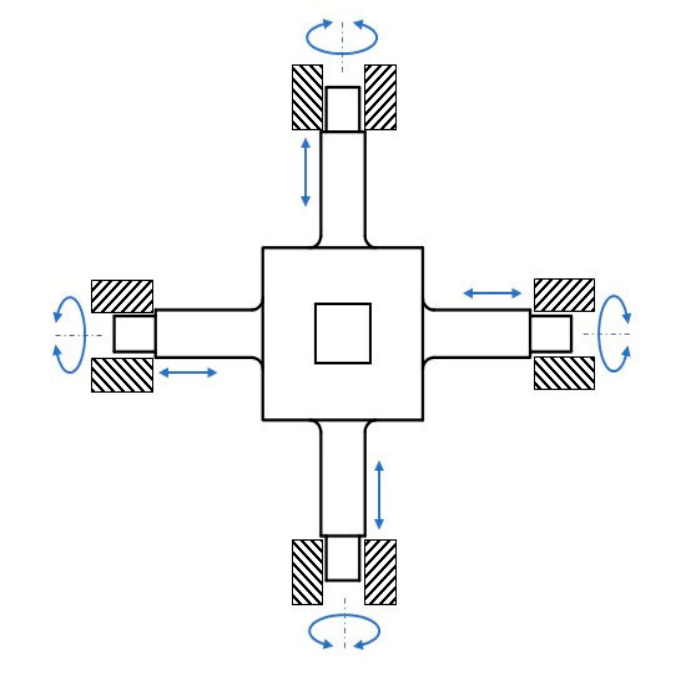
\includegraphics[width=\textwidth]{sliding_beam.png}
        \caption*{sliding joints}
    \end{subfigure}
    \caption{Example of flexible joined beams structures for multi-axial sensors.}
    \label{fig:flexible_beams}
\end{figure}

\begin{enumerate}[resume]
    \item Modal cross-beams
\end{enumerate}

With the advancement in computational power, the creation of mechanically decoupled solutions has become more accessible. 
In their study, Mayetin and Kucuk \cite{modal_sensor} developed a modal sensor with an average interference error of less than 3\%.
This approach allows for the replacement of failed structural elements, enhancing the overall reliability and longevity of the sensor.
\begin{figure}[H]
    \label{fig:modal_sensor}
    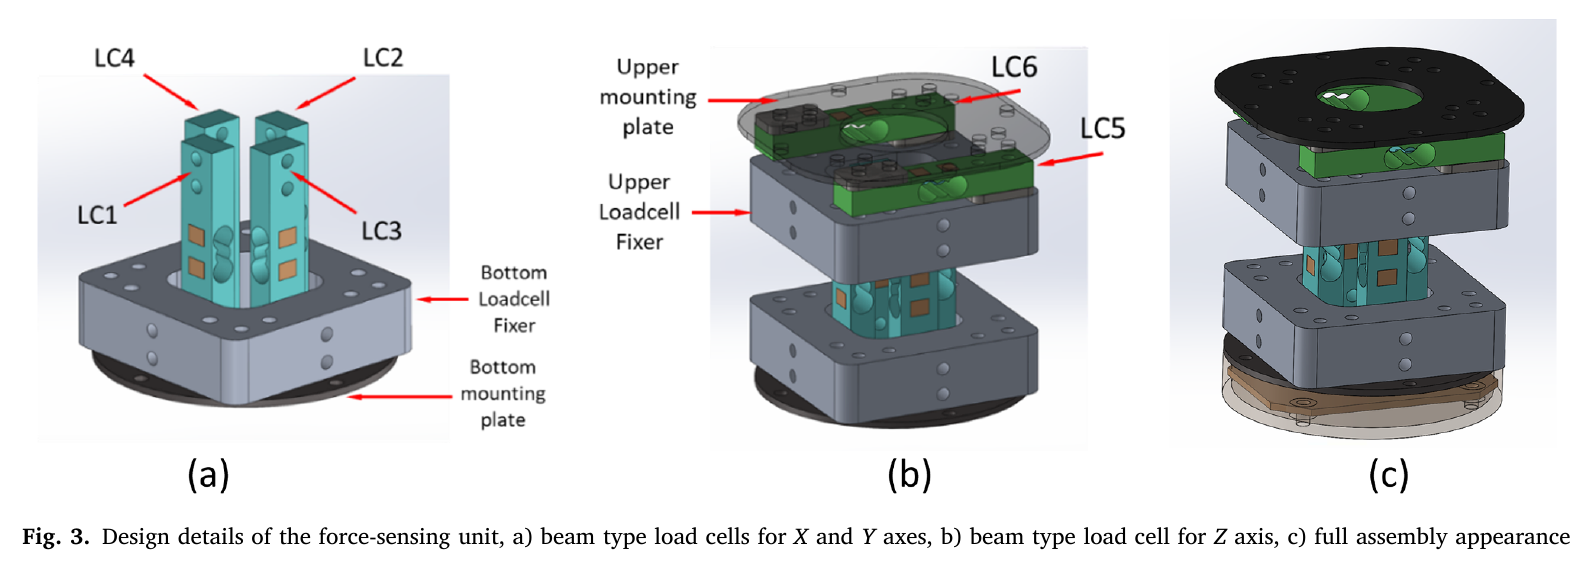
\includegraphics[width=\textwidth]{modal_sensor.png}
    \caption*{modal sensor from \cite{modal_sensor}}
\end{figure}

% \begin{enumerate}[resume]
%     \item Dual-layer cross-beams
% \end{enumerate} 

% Перед констракшеном

\section{Conclusion}
\label{lr_conclusion}
In this literature review, we have explored the research conducted by Hosseinabadi and Salcudean \cite{perfect_sensor} and the model proposed by
 \cite{my_love_pressure_photosensor} for a mechanically decoupled six DOF force sensor with low cross-coupling error and high resolution to scale 
 ratio of 0.0001\%. 
 Additionally, we have examined the 3-DOF force sensor structure proposed in \cite{modal_sensor}, 
 which features four independent beams with an average interference error of less than \( 3 \% \).

Building upon these previous studies, the current research aims to develop a mechanically decoupled modal structure for a six DOF force sensor,
utilizing the measurement cell invented by \cite*{my_love_pressure_photosensor}. 
The focus of this study will be on calculating the cross-coupling interference, resolution to scale ratio, and hysteresis of the sensor. 

% \cite*{optic_mirror}
% This enables the development of a versatile solution suitable for a wide range of loads. The design offers several benefits, including protection against electromagnetic interference, the ability to adjust the range of values by modifying the barrier, and cost-effectiveness and availability of the structural elements.
\chapter{Methodology}
\label{chapter:methodology}

\subfile{chapters/methodology/optical_modeling.tex}
\section{Electric Design}
\begin{figure}[H]
    \centering
    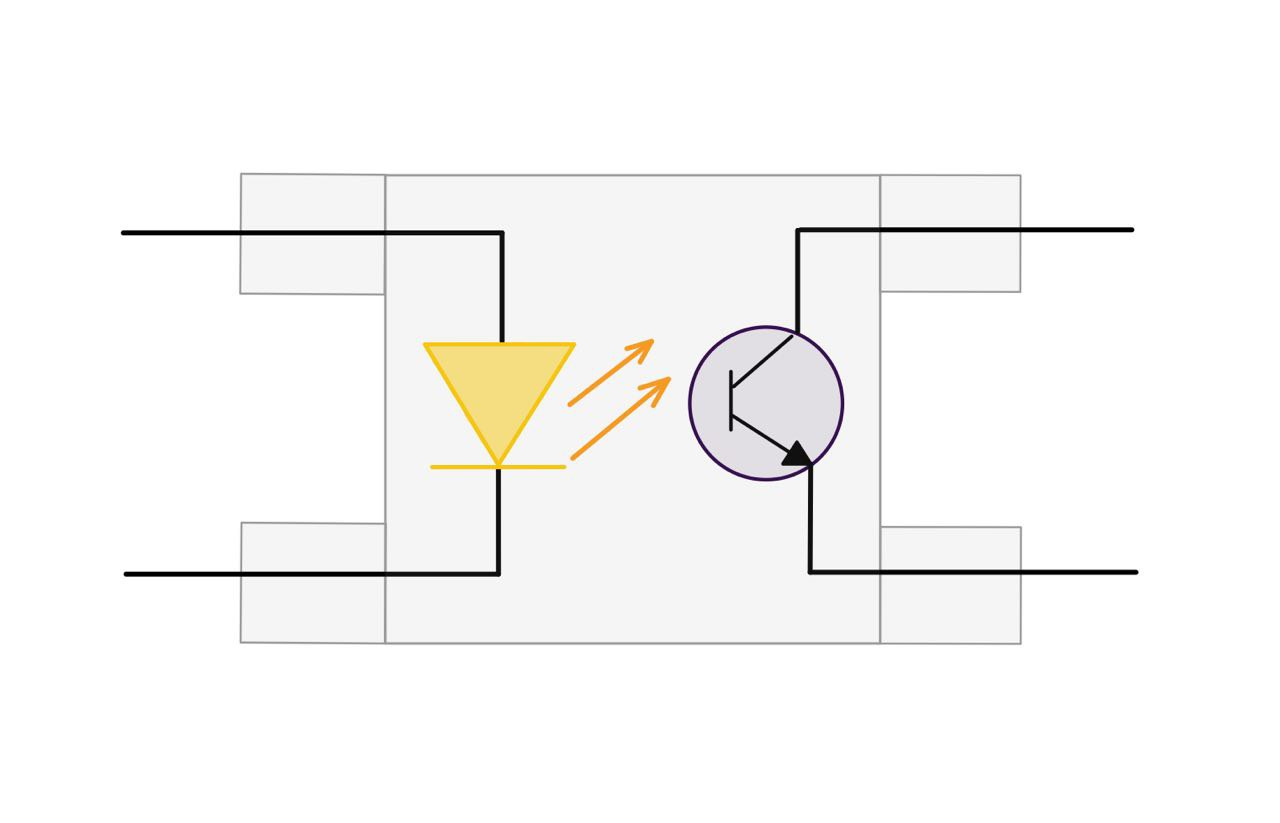
\includegraphics[width=\textwidth]{ED/optopair_scheme.jpg}
    \label{fig:optopair_scheme}
    \caption{General design of optopair sensor.}
  \end{figure}
\chapter{Implementation}
\label{chapter:implementation}

This chapter describes the theoretical aspects of six-axial optical force sensor development, the data filtration, communication protocols and the calibration process?

% ~\nameref{capter:literature_review}


% \chaptermark{capter:literature_review}
% This chapter covers theoretical aspects related to the translation of Java to EO, developed projections, and a description of the software project developed alongside this thesis.


% \section{Conceptual comparison of Java and EO}
% \label{section:conceptual_comparison}

% To start translating of one language into another, it is important to understand their differences. Even the same term may be interpreted differently by developers of several languages.

% \subsection{Paradigm}

% It is important to remember that in the past various languages, including Java, spoiled the original notion of the object-oriented paradigm. Thus, the object-oriented paradigm is interpreted differently by developers of different languages. Original implementation of object-oriented paradigm is present in Smalltalk \cite{smalltalk} and is focused on objects, not classes.

% Java implements a nowadays traditional OOP paradigm. The correct name of the paradigm would be \emph{class-oriented}, since developer has no access to objects, only to classes. This approach also strictly forces developers to put everything in classes or interfaces, which are the only available top-level constructs.

% EO is closer to the functional paradigm, with a focus on objects, as in the original object-oriented paradigm.

% \subsection{Visibility}
% % TODO: wrap this into some section/subsection.
% % TODO: maybe move part of this stuff to the EO overview chapter?
% Java has a strict visibility system that includes four levels described in
% subsection \ref{subsection:java_visibility}. EO, on the other hand, has no
% visibility system at all. Such a visibility system is hardly possible in EO given its dynamic nature, including dynamic typing, lack of object structure specification and unlimited access to the creation and modification of objects.
% These features are required to keep the language structure flexible enough to translate various languages into it.


% \subsection{Mutability}
% In Java, all variables are mutable by default (though it may be limited using final). EO has no built-in mutability, but it has workarounds for that in the standard library: \ff{memory} and \ff{cage}.


% \subsection{Programming style}
% Java has an imperative style --- developer writes a code that describes \emph{how} to do the task. Declarative style may be achieved using custom-implemented pair of executor and data structure, but it will not work soundly with libraries (both standard library and external libraries). Custom wrappers are needed to support libraries.

% EO has a declarative style --- developer writes \emph{what they want to achieve}, not how to achieve that. Imperative style may be achieved using a built-in atom named \ff{seq}, but because of the implementation nature, the scope of \ff{seq} is more restrictive than the object scope, e.g., it is not possible to declare variables inside.



% \section{Projections}

% This section will go over theoretical approaches of projecting Java source code into semantically equivalent EO source code.

% \subsection{Naming}
% Java and EO have different conventions for naming language components, and while Java does not enforce naming conventions, EO does. Consequently, name mapping has to be developed and be consistent across the translator to keep the result code working.

% Specifically: object and attribute names in EO can only start with lower-case letters and continue with upper/lower case letters, numbers, dashes or underscores. This differs from Java only in the first symbol, therefore, the solution is to prepend names with fixed text sequence.

% Also, EO has problems with attribute shadowing. Attribute shadowing is a feature of a language that allows redefining variables (attributes in EO terms) in nested scopes. This feature works in an unpredictable manner, especially considering the unstable nature of EO (it is still in the early stage of development and behavior changes frequently as of the time of writing this). Because of that, the translator avoids name duplication as much as possible. The first step to minimize such duplications is to prepend different types of source code tokens with different prefixes.

% As a solution to the attribute shadowing problem, the following mappings were developed:
% \begin{itemize}
%     \item class names are prepended with \texttt{class\_\_}
%     \item variables are prepended with \texttt{var\_\_}
%     \item arguments are prepended with \texttt{arg\_\_}
%     \item methods are prepended with \texttt{method\_\_}
% \end{itemize}


% \subsection{Constructors}
% Java, like many modern OOP languages, has class constructors. EO does not have classes, and thus the implementation of constructors is under full control of the translator. In the current form, Java constructors are mapped into function attributes with an extra \texttt{cons} name.


% \subsection{Overloading}
% Also, EO does not support method/constructor overloading and even does not have functions directly. They are simple objects, like everything in the language. Therefore, the name of methods/constructors are appended with type names, separated with \texttt{\_\_}. Generics information is omitted, as JVM does not have it as well.

% Example of resulting mapping considering everything above:
% \begin{ffcode}
% class A {
%   A(int member) {...}
%   void functionName(int arg1, Option<Value> arg2) {...}
% }
% \end{ffcode}

% \begin{ffcode}
% [] > class__A
%   [] > new
%     [] > this
%       [var__member] > cons__int
%         ...

%       [] > method__functionName__int__Option
%         ...
% \end{ffcode}


% \subsection{Expressions}
% Java provides a way to create complex nested and chained (separated with dot) expressions. These expressions can cause various side-effects in various order. 


% \subsubsection{Chained expressions}

% The tricky case is chained expressions. Due to EO's specific function calling approach, calling a method of a class instance requires passing that instance as the first argument, i.e. \texttt{obj.function(obj)}. This is effortless when single-expression statements are used, but chaining with a dot requires storing the intermediate object somewhere to be able to proceed in the chain.

% Consider the following Java example:

% \begin{ffcode}
%   var result = obj.setValue(value).computeResult();
% \end{ffcode}

% Here, \texttt{obj} should be passed between chained calls. To resolve this collision, it was decided to split each chain operation into a separate binding, and use them inside other bindings. This allows to abstract out the double use of the same value from higher-level abstraction. 

% Since internal operations do not act as dependencies to the outside of expression, their names are generated randomly and have a UUID format.

% The order goes from inside to outside, so dependencies of outer expression parts are already defined above, although it does not matter to EO, as an evaluation only starts in the \texttt{seq} block at the end of the function object.


% The example of EO code that corresponds to the above Java snippet:

% \begin{ffcode}
% ... > obj
% ... > value
% ...
% [obj] > <uuid_1>
%   seq > @
%     obj.setValue obj value
% [obj] > <uuid_2>
%   seq > @
%     obj.computeResult obj
% ...
% seq > @
%   ...
%   <uuid_2>
%     <uuid_1>
%       obj
% \end{ffcode}

% Although the EO variant takes considerably more code to do the same operation, the language was never meant for hand-writing code, only for translation from other languages.


% \subsubsection{Side-effects in expressions}

% Consider the following Java snippet:

% \begin{ffcode}
% var out = obj.setValue(obj2.setValue(obj2.getCount()).i++);
% \end{ffcode}

% It is different from the previous snippet by one feature --- post-increment operation, which is an in-place mutating side-effect.

% In this code, in given order, the following operations occur:
% \begin{itemize}
%     \item Function \texttt{getCount} of \texttt{obj2} is invoked and result is obtained 
%     \item Function \texttt{setValue} of \texttt{obj2} is invoked with the obtained value
%     \item \texttt{obj2} returns itself for further chained call
%     \item Property \texttt{i} of \texttt{obj2} is obtained
%     \item Property \texttt{i} of \texttt{obj2} is incremented by 1
%     \item Function \texttt{setValue} of \texttt{obj} is invoked with value obtained before increment, as this is value type, not reference type
%     \item The result of \texttt{setValue} is assigned to \texttt{out}
% \end{itemize}

% As it is seen from the list above, the order of execution does not correspond to the AST, in particular --- post-increment operation. This operation should have been placed before obtaining the result, as in pre-increment, to match the AST structure. This fact of altered order makes Java code hard to translate to EO, which does not have corresponding syntactic sugar, as well as value-typed variables.

% The general problem is causing side-effects from the expression: EO discourages any side-effect operations and only provides "gray" workaround atoms to mimic side-effects, to create a compatibility layer with side-effect-based programs. But since there are still no value types, we have to work around operations that rely on them with custom logic (i.e., creating a new variable).

% Considering methods described above, we can obtain the following EO mapping:

% \begin{ffcode}
% ... > obj
% ... > obj2
% ...
% [obj] > <uuid_1>
%   memory > result
%   seq > @
%     result.write
%       obj.getCount obj
%     result
% [obj arg] > <uuid_2>
%   seq > @
%     obj.setValue obj arg
% [obj] > <uuid_3>
%   memory > result
%   seq > @
%     result.write
%       obj.i
%     obj.i.write
%       add
%         obj.i
%         1
%     result
% [obj arg] > <uuid_4>
%   seq > @
%     obj.setValue
%       obj
%       arg
% ...
% seq > @
%   ...
%   <uuid_4>
%     obj
%     <uuid_3>
%       <uuid_2>
%         obj2
%         <uuid_1>
%           obj2
%   ...
% \end{ffcode}


% Notice how post-increment was implemented in \texttt{<uuid\_3>}: new \texttt{memory} object (think of it as of cell that can store some value) is created, the current value is copied there, and then the original object's value is updated.

% The same approach is used everywhere where value types are used (for Java, the list includes \texttt{int}, \texttt{long}, \texttt{short}, \texttt{char}, \texttt{float}, \texttt{double}). In this case, it is used in \texttt{<uuid\_1>}. This provides a reliable way to ensure that the original value will not be changed by subsequent function calls, as it is not changed in Java.


% \subsection{Resolving Java compound names}
% Java has a very unfortunate feature of referencing nested classes/members: every token is separated with a dot in any case. Therefore, it is impossible to tell which exact operation is represented by a particular dot: is it a part of a package name, referencing a class from a package or referencing a member of a class.

% To determine the operation of the compound name, the import block is analyzed:
% if the line from the Java import block (excluding the last part, either \texttt{*} or class name) is a start of the compound name, parts of the package are not altered in the EO compound name; the file referenced by the package name is loaded, parsed and analyzed. parts that correspond to class names are prepended with \texttt{class\_\_}, parts that correspond to variable names are prepended with \texttt{var\_\_}.


% \subsection{Mapping classes}
% % <insert reference to conference paper>
% % <copy from J2EO paper>

% Class bodies are fairly straightforward to translate.
% \begin{itemize}
%     \item class is an object with all static members and static methods, plus \texttt{new} object factory and \texttt{cons<n>} constructors. It also decorates the superclass, inheriting its static members and methods.
%     \item \texttt{new} method decorates superclass'es \texttt{new} object and defines class members with their default values over that.
%     \item \texttt{cons<n>} method that contains corresponding Java constructor code.
% \end{itemize}

% What poses a challenge is an inheritance, especially multiple inheritance (implemented via interfaces in Java). There are still no observed approaches to map interfaces in the project, so they will be skipped for the time being. The focus will be on mapping classes.

% Superclass is written to \texttt{super} attribute of an instance during its creation.


% Below is an example of class mapping:

% Original Java code snippet:
% \begin{ffcode}
% class A {
%   int i = 42;
%   int getI() { return i; }
% }
% class B extends A {
%   int i = 1;
%   B() { super(); i = 2; }
%   int getI() { return i; }
%   int getSuperI() { return super.i; }
%   int setSuperI(int i) { super.i = i; }
% }
% \end{ffcode}

% Produced semantically-equivalent EO code:
% \begin{ffcode}
% [] > class__A
% [] > new
%   [] > this
%     memory > i
%     [this] > getI
%       this.i > @
%   seq > @
%     this.i.write 42
%     this
% [this] > cons1
%   this > @

% [] > class__B
% [] > new
%   [] > this
%     class__A.new > super
%     super > @
%     memory > i
%     [this] > getI
%       this.i > @
%     [this] > getSuperI
%       this.super.i > @
%     [this i] > setSuperI
%       seq > @
%         this.super.i.write i
%         this
%   seq > @
%     this.i.write 1
%     this
% [this] > cons1
%   class__A.cons1 this > this2
%   seq > @
%     this2.i.write 2
%     this2
% \end{ffcode}


% \subsection{Mapping interfaces}

% EO's feature that allows the extension of other objects is decoration. Decoration only allows simulation of singular inheritance, though. Java 8 brought default methods to interfaces --- which essentially facilitated multiple inheritance. This does not fit into $\varphi$-calculus, so can only be worked around, not natively implemented.

% The current solution simply ignores interfaces, since mostly they only facilitate static checking when data hiding is needed. This approach behaves incorrectly with default methods, though.


% \section{J2EO implementation overview}

% In addition to theoretical mappings, the result of work on the thesis is a software project named J2EO. The project is written in Java/Kotlin with parser implemented in ANTLR \cite{antlr_website}. 

% The flow of a single Java file through different modules is shown below.

% \begin{figure}[H]
%   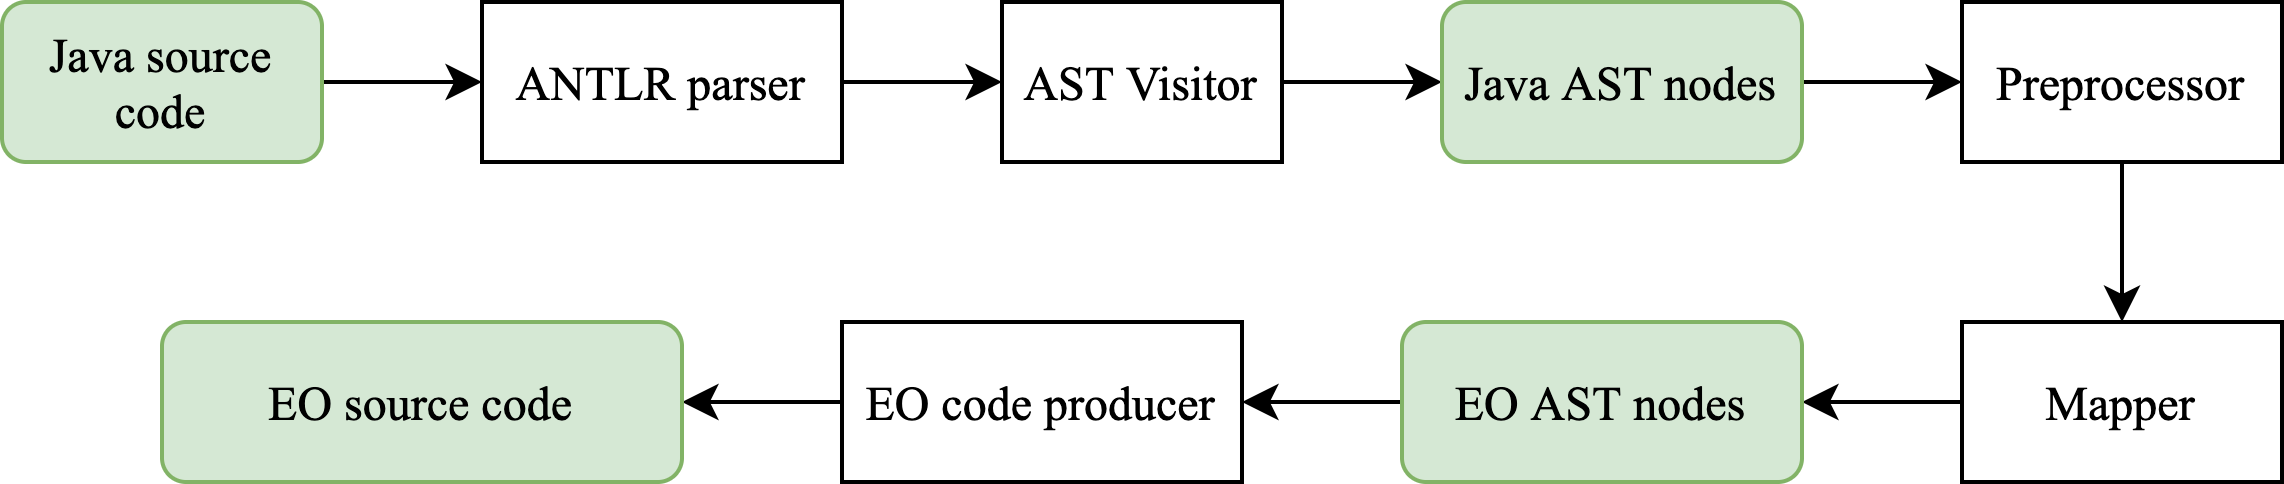
\includegraphics[width=1\textwidth]{j2eo_structure.png}
%   \centering
%   \caption{Processing of a single Java file through the J2EO pipeline}
%   \label{fig:j2eo_flow}
% \end{figure}

% The wrapper that handles I/O, execution of pipeline and other routine tasks is not covered by this text.

% The following part of the section describes each of the steps in more detail.

% \subsection{ANTLR parser}
% Java parsers for modern versions of the language are hardly available on the Internet. The only parser that fully covers Java 17 is implemented in ANTLR and is available on GitHub \cite{antlr_java_parser}. Slight modifications are required to make it work for J2EO's use case.

% \subsection{AST Visitor}
% This pipeline step executes ANTLR parser and visits each node to generate an internal Java AST node. This step is required because ANTLR itself does not generate AST nodes, it only provides context which can be used to obtain parts of the tree.

% \subsection{Preprocessor}

% The preprocessor applies naming convention patches to the code. This step includes prefixing of identifiers, renaming imports to suit EO conventions and other semantically-neutral changes.

% \subsection{Mapper}

% This is the core pipeline step, which produces EO AST nodes from preprocessed Java AST nodes. The methodology of projection of AST nodes is provided in the above section.

% \subsection{EO code producer}

% The final step of the pipeline is to produce source code from the EO AST. This part is implemented as Kotlin extension functions which add methods to EO AST nodes in a non-invasive manner.

% \subsection{Summary}

% All pipeline steps above are implemented in a functional style. Thus, none of the functions utilize the shared mutable state, which makes it possible to parallelize the translation of files. The parallel version of J2EO was successfully tested.

% J2EO project is open-source and is available on GitHub \cite{j2eo_repo}. Anybody can use it and contribute to it.





\chapter{Results and Discussion}
\label{chapter:results_and_discussion}

\section{Results}

% The result of this thesis is a part of the software program J2EO written in Java/Kotlin. The implemented part includes EO Abstract Syntax Tree (AST), an algorithm that prints EO AST to the source text file, and an algorithm that translates selected Java AST nodes to EO AST.

% % TODO: move to the introduction?
% The main use case for J2EO is to translate real-world Java projects to EO to later perform static analysis with other Polystat projects. Thus, it is important to translate large projects without failures and maximize the amount of translated Java features. Producing full semantically-equivalent code is not a requirement for static analysis.

% As the benchmark for result assessment, I have picked several big projects heavily used in production systems.

% The table of used projects with their corresponding actual commit hashes is listed in \tab{table:benchmark_projects}:

% \begin{table}[H]
%     \centering
%     \begin{tabular}{| c | c | c | p{5cm} |} 
%         \hline
%         Project & Java version & LoC & Actual commit hash \\
%         \hline
%         Hadoop \cite{hadoop_repo} & 8 & 1631465 & ec0ff1dc04b2ced199d7- 1543a8260e9225d9e014 \\
%         \hline
%         Kafka \cite{kafka_repo} & 8 & 499373 & f36de0744b915335de6b- 636e6bd6b5f1276f34f6 \\
%         \hline
%         J2EO \cite{j2eo_repo} & 17 & 41200 & a762a903eb55f3e11403-d4630654f4c89397d75a \\
%         \hline
%     \end{tabular}
%     \caption{Java projects used for benchmarking}
%     \label{table:benchmark_projects}
% \end{table}

% The version of J2EO used is 0.5.3 and is present on the GitHub repository \cite{j2eo_repo} of the project.

% Lines of Code (LoC) metric was computed using \ff{cloc} utility \cite{cloc} and includes only physical Java lines, excluding empty lines and comments.

% Given software versions and commit hashes allow readers to reproduce results given in the text on their own machine.

% \subsection{Designed projections}

% Theoretical projections for many Java constructs and features are developed as a part of this thesis. The full list is present in Chapter \ref{chapter:implementation}.

% % write about upcoming paper

% \subsection{Implemented projections}

% As of the time of the writing, projections implemented in J2EO cover mapping of classes, their static and non-static members, static and non-static methods, support for most of the statements which make sense to statically analyze. Any project structure is parsed correctly, so both Maven and Gradle projects with arbitrary directory structure may be passed as input.

% Priority of projection implementation was actively discussed with the analyzer development team, so included mappings are actual for the future development of the entire super project.

% The supported version of Java is 17 and given it is backward compatible, any lower-version projects are also supported. Several entries in the benchmarking tables confirm that.

% \subsection{Assessment of results}

% Objective assessment of results is not possible as of the time of writing, because Polystat analyzer is still in early stages of development and thus no full pipeline of analysis exists.
% The main method of assessment used is to translate large Java projects and check the correctness of produced EO files by hand. Benchmarked projects provide a several million lines of code and the fact that translation successfully terminates is promising for the future of the project.


% \section{Discussion and Conclusion}

% The text presented an overview of used technologies, including Java, EOLANG and $\varphi$-calculus, then provided an assessment of these technologies for the goals of the project, theoretical projections of constructions between the source and target languages, and finally described the implementation of the tool itself.

% The J2EO project already covers a significant range of Java features, facilitating the future development of the Polystat analyzer. Since Polystat heavily depends on the output of transpilers, its development was stalled for a long period and thus no rich analysis results are produced as of the time of writing.

% J2EO/Polystat combination is still under active development. However, according to the results of J2EO, EO provides a necessary base for the representation of other languages. This combination has a solid chance to become competitive with other popular Java static analyzers, such as PMD, SpotBugs, and IntelliJ IDEA built-in static analyzer (which is not available standalone).

% The ongoing research on the Java to EOLANG projections and J2EO translator tool will be released to academic community in the upcoming paper later this year.

% \section{Acknowledgements}
% \label{acknowledgements}

% Big thanks to Nikolai Kudasov for help and consultation related to EOLANG, my other team members, including Eugene Zouev, Egor Klementev, Ilya Miluoshin for collaborative work on J2EO, Yegor Bugayenko for releasing phi-calculus and EOLANG compiler, the open-source community for contributing to EOLANG repository and Rabab Marouf for teaching the Academic Writing course.

% \include{chapters/acknowledgements.tex}

%% REFERENCES
\printbibliography[heading=bibintoc,title={Bibliography cited}]
% \include{chapters/appex}
\end{document}